\section{Experiments}
\label{sec:experiments}

In this section, we discuss results obtained using the previously described deformation model.
We first test the model on handwritten character recognition, with the
aim of assessing its utility for discriminative tasks. 
Later we test the generative aspect of our model, through two
experiments: (1) sampling new images of digits, and (2) reconstructing
human faces.


\subsection{Handwritten Digit Recognition}
On the popular MNIST~\cite{MNIST} dataset, several state-of-the-art
algorithms produce error rates of approximatelyt $0.5\%$,
close to that of humans.
Our goal here is two-fold:
(1) to compare the performance of current best algorithms in estimating
deformations, and
(2) to show that a structured deformation model can lead to
improvement on generalizability, making it possible to maintain an
effective model with a small number of prototypes.


% So far, the three most successful algorithms are Support Vector
% Machine (SVM), Convolutional Neural Nets (CNN) and K-Nearest Neighbor
% (KNN) with well engineered features and distance functions.
% The former two algorithms, SVM~\cite{VSVM} and CNN~\cite{CNN}, try to form highly
% nonlinear boundary between different classes in the appearance model
% by high order polynomial kernels or by broad and deep nets.
% In order to capture the rich local deformations of handwritten digits,
% both algorithms have to add many synthetic images after certain
% deformation which greatly prolong the training process.

For digit recognition, we compare with three popular methods:
direct matching using Euclidean distance (L2), Image Distortion Model
(IDM)~\cite{IDM}, and Tangent Distance (TD)~\cite{TD}, 
Particularly, the latter two algorithms essentially build local
deformation modelsm around each training image.

We note that the training samples in MNIST are very dense, to the
extent that most testing samples have a very close match in the
training set. Therefore, with the use of the whole training set,
even simple Euclidean matching can achieve very good performance.
To differentiate between the generalizability of different methods,
we compare them using sub-sampled training sets of different sizes. 
%
Figure~\ref{fig:char_reg} shows that when the training set is small,
all methods make a considerable amount of errors, and the error rates
decrease as the training set grows. We can see that with a structured
deformation model, the error rate yielded by the proposed method
clearly drops faster than that by other methods. This is partly
ascribed to the fact that statistical strength is shared among local
models via parallel transport constraints.
\begin{figure}[t]
    \centering
    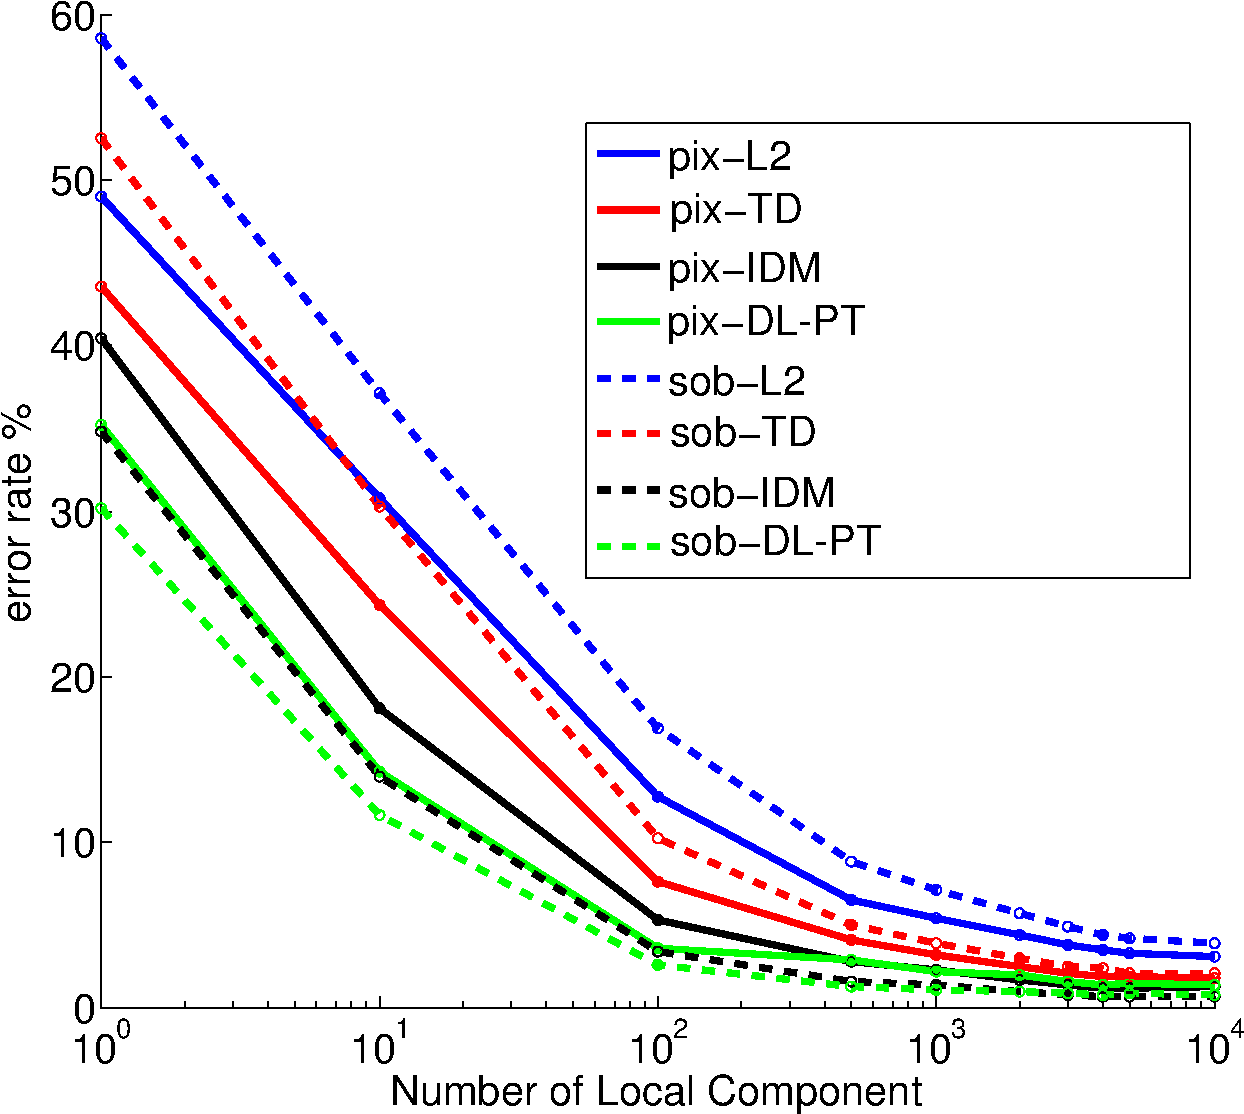
\includegraphics[height=0.7\columnwidth]{figs/f1_err1.pdf}
    \caption{Filled Line: Recognition error on MNIST dataset with pixel intensity as the feature;
      Dashed Line: Recognition error on MNIST dataset with response from Sobel filter as the feature.}   
    \label{fig:char_reg}
\end{figure}


\subsection{Image Synthesis}
%
While many image synthesis experiments are designed to demonstrate
super resolution results which are appealing from a human perceptual
standpoint, our primary purpose here is different. Rather, we wish to
show that the basis learned basis, which is shared across the manifold, are meaningful
from a geometric perspective.

\subsubsection{Digit Synthesis.}
%
For example, given the digit manifold learned from MNIST dataset, we are now able
to synthesize new images of digits by applying randomly sampled action
coefficients to randomly sampled prototypes.  In
Figure~\ref{fig:char_syn}, we show the randomly sampled prototype of
each digit in the first column and synthesized new digit images in the
rest of each row. One can see that the synthesized images
generated by integrating along the geodesic of the manifold cannot be
explained by global affine deformation. For example, in the row of digit two, we
can see that there are some basis related to the size of the lower
left circle of the digit.
\begin{figure}[t]
    \centering
    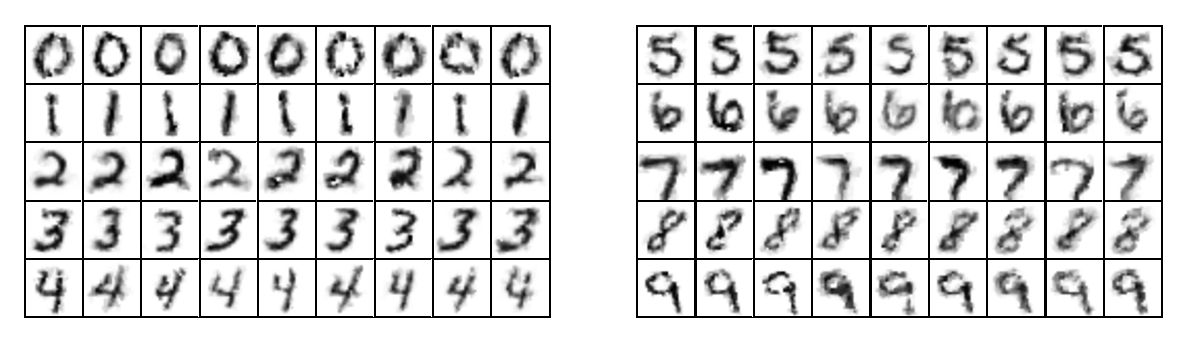
\includegraphics[height=0.28\columnwidth]{figs/digit_table.pdf}
    \caption{Synthesized digits from the learned digit deformation manifold. 
The first digit in the row is the prototype; 
the rest are locally deformed from the prototype with a random coefficients of the learned basis}
    \label{fig:char_syn}
\end{figure}

\subsubsection{Face Reconstruction.}
%
In addition, we learn a face manifold using
the face dataset of Brendan Frey, containing around
2,000 20 by 28 gray scale images of Frey's face in different
expressions and angles of view.  For this experiment, we first learn
the commonly shared basis to contruct the manifold from 1,000 sampled
images.  Then, for a separate set of randomly sampled 500 testing images,
we try to see how close they can be projected onto the manifold.  We
tested three different algorithms for reconstruction: nearest training
image in Euclidean metric, closest projection onto tagent spaces and
closest projection onto our connected deformation manifold with shared
basis.  Again, we test our results with a varying number of
prototypes. Shown in Figure~\ref{fig:face_syn}, we can see that the in
terms of both Euclidean distance and PSNR ratio, the reconstruction
from the manifold with a learned shared basis is consistently better than
those learned independently from training examples. Note that the images
are by themselves small and most reconstruction errors are not human
detectable. Consequently, we do not show the reconstructed faces.

\begin{figure}
    \centering
    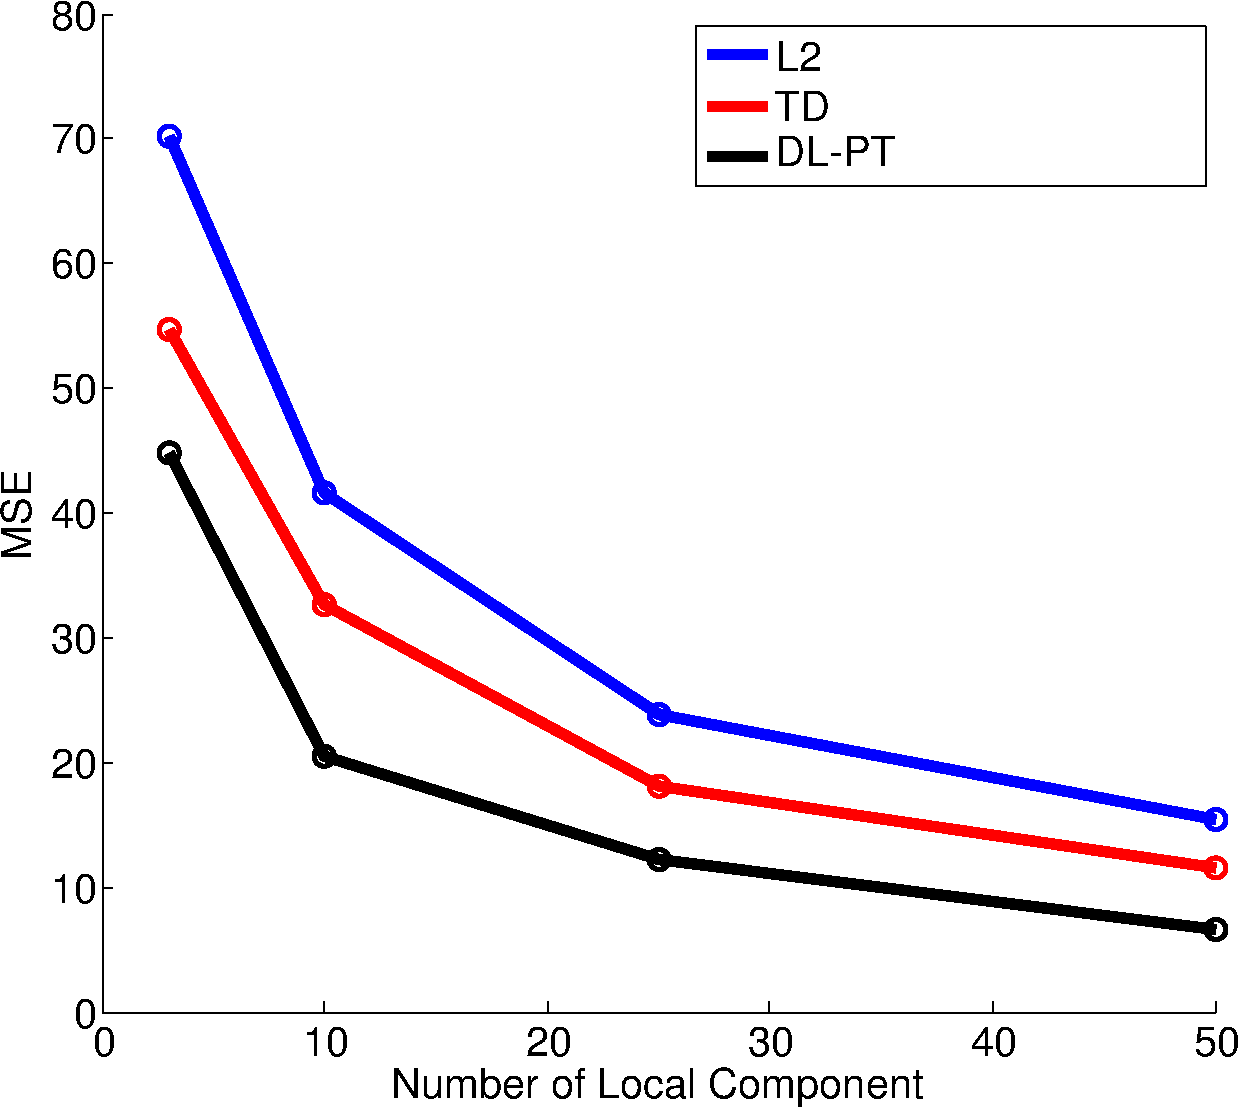
\includegraphics[height=0.4\columnwidth]{figs/f3_mse.pdf}
    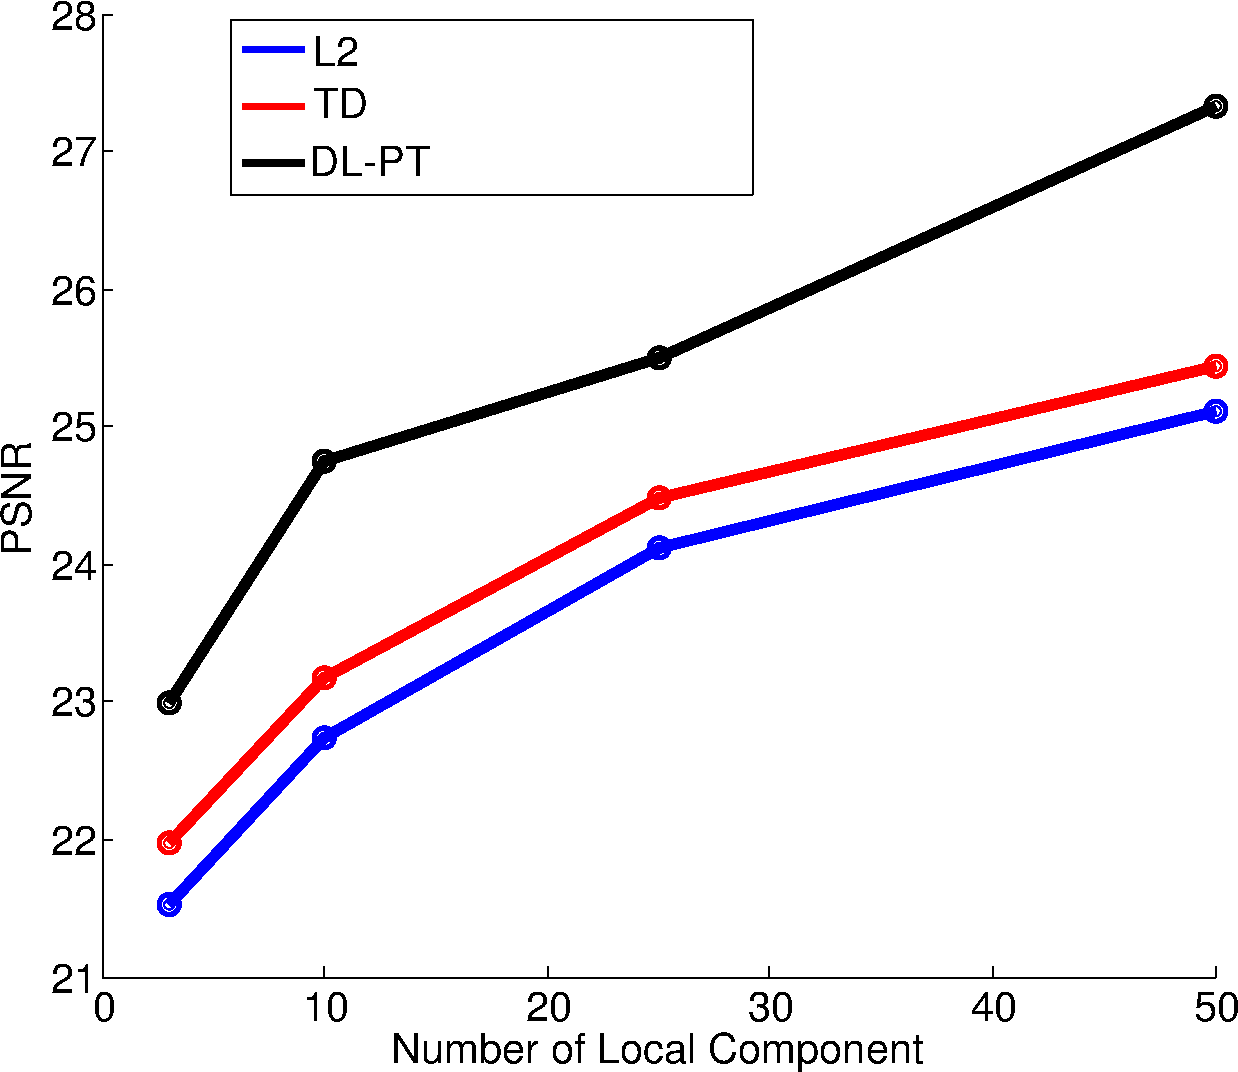
\includegraphics[height=0.4\columnwidth]{figs/f3_psnr.pdf}
    \caption{Comparison of reconstruction performance on face synthesis.}
    \label{fig:face_syn}
\end{figure}

%%% Local Variables:
%%% TeX-master: "main_paper"
%%% End:
